\chapter{Introduction}\label{chap:introduction}

\chapterQuote{\textit{``Ludwig Boltzman, who spent much of his life studying statistical mechanics, died in 1906, by his own hand. Paul Ehrenfest, carrying on the work, died similarly in 1933. Now it is our turn to study statistical mechanics.''}}{--- \textit{States of matter}, David L. Goodstein}

\chapterAbstract{T}{he purpose of this book is to present our work in Knowledge Graph reasoning. This chapter provides the required information for the reader to follow the topics discussed in this dissertation, it is structured in the following sections: 

Section~\ref{sec:intro-context}, contains; 
Section~\ref{sec:intro-rationale}, holds; 
Section~\ref{sec:intro-summary}, focuses on;
Section~\ref{sec:intro-collabs}, showcases,
Section~\ref{sec:intro-structure}, describes the structure of the rest of this book.}

\section{Research context}\label{sec:intro-context}


% Problems that arise from that,
 
% KG completion and reasoning context.

% Machine Learning
% Reinforcement Learning as a solution,
% how Rl applies KG reasoning techniques


In recent years available information online has increased 60.000\%, from a modest 2 zettabytes ($10^{12}$ gigabytes) up to an estimate of 120 by the end of 2023\cite{}. The sheer volume of information generated on a daily basis calls for a structured and networked storage solution made possible by Knowledge Graphs, which rise to popularity was all but inevitable. These data structures hold information from multiple domains by using triples, two information nodes representing concepts connected by an edge representing a relationship between them, this relation can be either directional or linear. This form of representation gives them a graph-like structure containing a web of facts with a high degree of connectivity, offering complex reasoned chains of information in an effective way.

\begin{figure}[!htp]
    \centering
    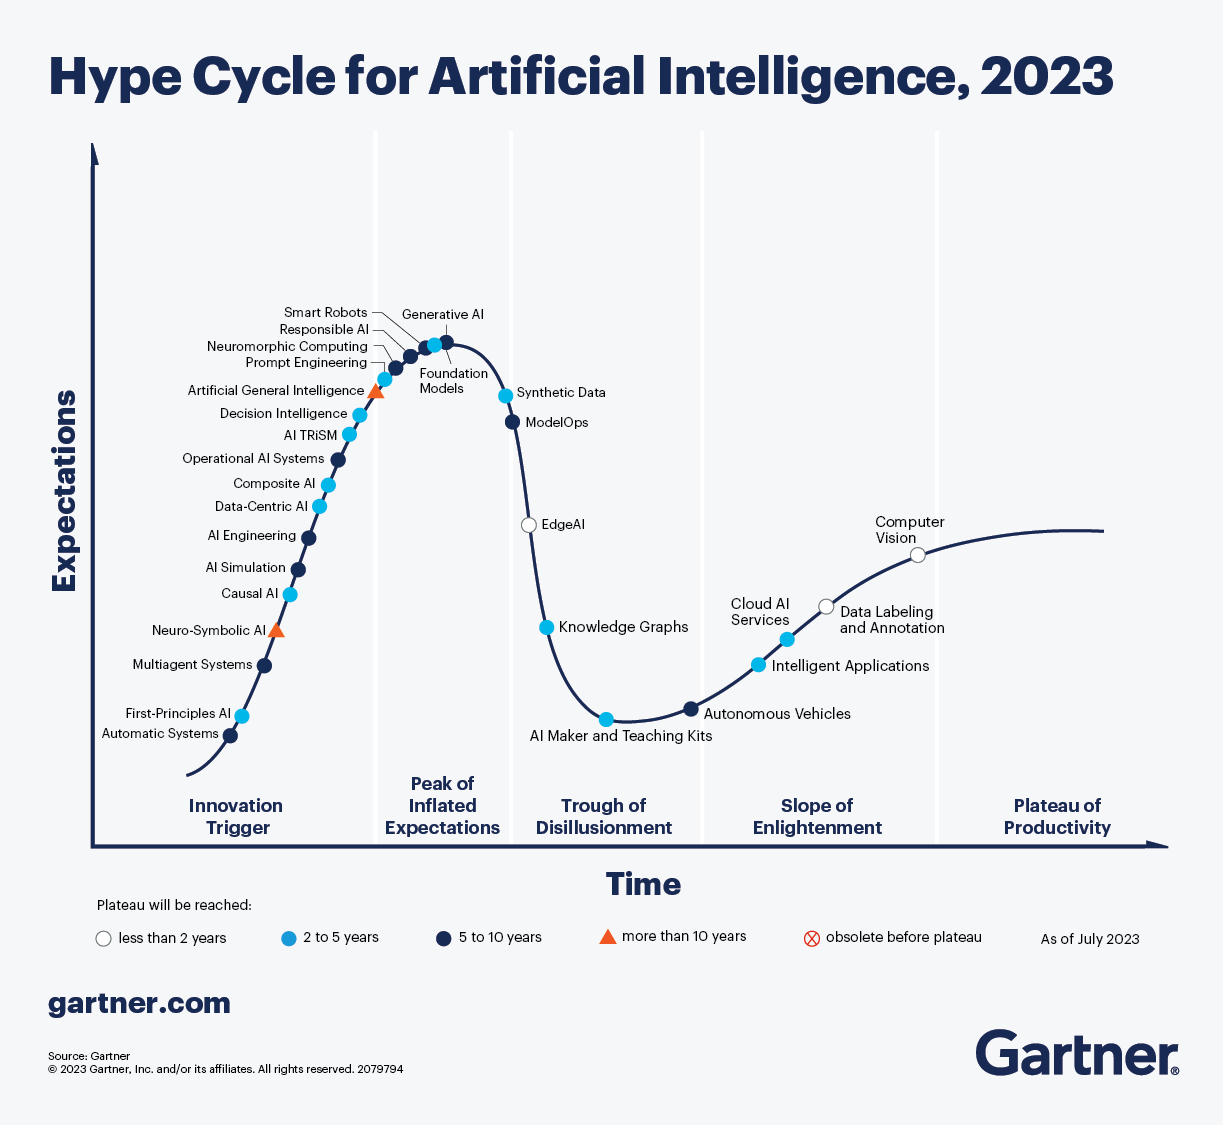
\includegraphics[width=\textwidth]{fig/intro/Gartner_2023.png}
    \caption{Gartner's 2023 hype chart for artificial intelligence.}
    \label{fig:garter-chart}
\end{figure}

The Garter institution situates Knowledge Graphs in the middle of their life cycle (cf. Figure \ref{fig:garter-chart}) meaning they can still benefit from active research and development and are still in their infancy in regards to their widespread applications in a multitude of fields. Some of the most notable fields and Knowledge Graphs corresponding to each of them are:
\begin{itemize}
    \item \textbf{Enciclopedic} KGs compile factual knowledge facts or events sourced from different domains, some examples are DBpedia\cite{auer2007dbpedia} which compiles the knowledge found in Wikipedia articles, Freebase\cite{bollacker2007freebase} which combines automatic processes from multiple sources as well as user contributions to wrangle up its data or YAGO\cite{suchanek2007yago} which adds a layer of complexity by adding temporal and geographical information to Wikipedia facts.
    \item \textbf{Linguistic} KGs compile facts about language and add a layer of information in the form of ontologies or external features on top, the most notable of these is WordNet\cite{miller1995wordnet} which provides hyponym and synonym relationships between words of the English language.
    \item \textbf{Enterprise} KGs support tech sector companies in their endeavors. The origin of Knowledge Graphs is found in this classification; the Google Knowledge Graph (GKG) \cite{steiner2012adding} boasting an impressive 800 billion facts on 8 billion entities. It compiles multi-domain information in order to rapidly respond to one of the many user queries made through their browser per day. 
    % Some other notable examples are Facebook's propietary KG, which holds information about its userbase's connections and likes in order to suggest new friends or groups.
\end{itemize}

Knowledge Graph construction is generally an automatic task since the large volume of data they hold is put off the range of human processing without it being an exceptionally arduous process, however, there are some notable exceptions such as the high-quality datasets that were constructed through crowdfunding efforts, Freebase\cite{bollacker2007freebase} and Wikidata\cite{vrandevcic2014wikidata}, automatic KG construction typically relies on semi-structured\cite{lehmann2015dbpedia} information ranging from XML type documents and html tables to plain text articles with a well-organized title structure.
Data Extraction from these sources has evolved over time from information extraction systems driven by designated rules or clustering \cite{yates2007textrunner, etzioni2004web}, to the current approaches such as, entity recognition\cite{huang2015bidirectional, ma2016end}, typing\cite{xu2018neural, ren2016label} and linking\cite{ganea2017deep, le2018improving} or relation extraction and curation\cite{zeng2015distant, zhou2016attention}. 

These methods of automated construction allow for a massive volume of data to be processed, however, they present several limitations.
First, the information they are built upon may be interpreted and linked erroneously or simply by being demonstrably wrong \cite{martinez2020information}, leading to incorrect facts being present in a KG. Second, Knowledge Graphs built from the same source might not be equal rendering them incompatible, they could represent the same facts with different nomenclature because they used a different schema to link that information \cite{choi2006survey}, meaning that joining Knowledge Graphs is never a trivial task.
Finally KGs are generally missing information since....

\todo{go into depth about kg completion here.}



% Those automated means of construction allow KGs to contain very large amounts of information, however, they introduce a number of issues. First, two Knowledge Graphs that are constructed separately are generally not mutually compatible, either because they represent the same concepts in different ways \cite{ren2022}, or just because they have a different language or modality \cite{javed2021,guo2021}. Second, the information they are built upon may be incorrectly interpreted or simply factually wrong \cite{paulheim2017}, leading to incorrect facts being present in a KG. Finally, fully automated KG construction methods are prone to missing information present in the original source \cite{bordes2014b}. Additionally, no single source of information, or combination of them, explicitly contains all pieces of information about a single domain. For these reasons, Knowledge Graphs are fundamentally incomplete. The process of finding facts missing from a KG and using them to complete it is a task known as Knowledge Graph completion, and it is the focus of this dissertation.

% In the literature, KG completion has been approached in a number of different ways, however, most existing proposals can be classified in one of three ways \cite{shen2022overview}. Some authors propose using logical rules to find missing facts, which analyze the existing information patterns in a Knowledge Graph to deduce rules that can then be used to generate further knowledge \cite{jiang2016, galarraga2015, galarraga2013, wang2015, richardson2006, kuzelka2019, yang2017, sadeghian2019, minervini2018, wei2015}. Other authors have proposed using a variety of embedded knowledge representations, which provide a more compact way to represent the information in a KG and can be leveraged to generate more knowledge \cite{nickel2011, jenatton2012, garcia-duran2015, yang2014, tay2017, trouillon2016, bordes2013, wang2014, lin2015, do2018}. A third line of techniques focuses on using information that can be found in the paths that exist between entities in a KG, and in the contexts of the entities themselves \cite{lao2011, gardner2015, gardner2013, nastase2019, gu2015, toutanova2016, jiang2017, lei2019, bansal2019a2n, wang2019}. In our proposal, we extend this third line of work.

% Regardless of how they are classified, most existing KG completion proposals have a very limited ability to actually generate new knowledge: they either rely on a set of candidate facts being provided to them for evaluation, or require a pre-made combination of one entity and one relation to be specified \cite{shen2022overview}. For this reason, although they may yield satisfactory metrics in a theoretical evaluation, they are of little practical use. A separate challenge in KG completion is to efficiently materialize a set of candidate triples of a reasonable size, that aims to minimize the amount of clearly incorrect triples it contains while retaining as many correct ones as possible. A much smaller body of work can be found in this regard \cite{shi18, zhang2019, omran2018}, even though it is a key step for completing a Knowledge Graph.

\section{Research rationale}\label{sec:intro-rationale}
In this section, we present the hypothesis that has motivated our research work in the context of Knowledge Graph reasoning and state our thesis, which we prove in the rest of the dissertation.

\subsection{Hypothesis}
% Nowadays, there is an increasing interest of individuals, organizations and companies in using Knowledge Graphs to represent information about a certain domain and to exploit said KGs to provide services. In the present day, practical applications such as question answering \cite{singhal2012}, product recommendations \cite{zhang2021, palumbo2020}, data retrieval \cite{wise2020} and meta-research \cite{dessi2022cskg,angioni2021} already rely on Knowledge Graphs. However, these applications need the data present in KGs to be as complete as possible, which makes it necessary to expand them after their creation.

% According to the previous argumentation, we conclude that our hypothesis is the following:

% \hypthesis{Knowledge Graphs provide value to individuals and companies alike by supporting applications that are widely used today, and their usefulness is likely to keep growing. Due to their incompleteness, there is a need to refine them and find the information that they are missing in order to expand them.} 

\hypthesis{Hypothesis goes here.}

\subsection{Thesis}
% There already exist a number of techniques that can be applied to perform Knowledge Graph completion, e.g., \cite{jiang2016, galarraga2015, galarraga2013, wang2015, richardson2006, kuzelka2019, yang2017, sadeghian2019, minervini2018, wei2015, nickel2011, jenatton2012, garcia-duran2015, yang2014, tay2017, trouillon2016, bordes2013, wang2014, lin2015, do2018, lao2011, gardner2015, gardner2013, nastase2019, gu2015, toutanova2016, jiang2017, lei2019, bansal2019a2n, wang2019}. Unfortunately, they do not fulfill a number of requirements for their application to large Knowledge Graphs. Those that rely on extracting and applying rules suffer from a particularly poor scalability, which has been acknowledged in the literature \cite{galarraga2013}. A large number of proposals use latent representations such as tensors, or entity or relation embeddings. While they can be effective, they are hindered by the fact that these representations must be obtained beforehand, which is a very computationally intensive task, and they must be updated entirely when a new entity or relation is introduced to the graph, which is a frequent event. Furthermore, many other proposals for KG completion need to access external or manually-provided information, making them not fully automatic or self-contained.

% In light of the previous reasoning, we conclude that our thesis is as follows:

% \hypthesis{In the context of Knowledge Graph completion, it is possible to overcome the problems of existing proposals and develop a new one to automatically complete the missing information in a large KG, in a way that does not rely on external information or alternative representations, but that still achieves a high effectiveness.}

\hypthesis{thesis goes here.}


\section{Summary of contributions}\label{sec:intro-summary}
To prove our thesis, we have devised SpaceRL, a XXX YYY program that does stuff.:

% \begin{itemize}
%     \item \textbf{CHAI}, a technique that is able to quickly filter out a large amount of candidate triples, leaving only the most promising ones. To do this, CHAI generates a number of rules that determine which triples have a higher chance of representing correct facts and deserve further evaluation, and which ones are most likely wrong and should be discarded immediately. Each of these rules is generated in an iterative manner, evaluating which continuation for it is the most promising. After a rule has been expanded, it is assessed again to determine whether it needs to be expanded further or not.\\
    
%     Regarding this contribution, the article that describes it \cite{borrego2019} was accepted and presented at K-CAP 2019.\\

%     \item \textbf{CAFE}, a technique that is able to learn what constitutes a correct and a wrong fact, and thus can select only the correct triples provided by CHAI, which can then be added to a KG, completing it. CAFE relies upon a set of neighborhood-aware features that are able to accurately characterize the neighborhoods of a pair of entities. It then uses these features to transform all triples it is provided into feature vectors, and trains a set of neural classification models to learn to distinguish between correct and incorrect knowledge.\\
    
%     Regarding this contribution, the article that describes it \cite{borrego2021} was published in the EAAI journal.\\

%     \item \textbf{SciCheck}, a proposal that is specifically designed to complete scientific Knowledge Graphs. Due to the particularities of these KGs, regular KG completion proposals do not provide satisfactory results. SciCheck overcomes these issues by considering the semantic similarities of the research concepts in a KG and by leveraging the rich ontologies that such KGs usually have.\\
    
%     Regarding this contribution, the article that describes it \cite{borrego2022} was published in the IEEE Access journal.

% \end{itemize}

\section{Structure of this dissertation}\label{sec:intro-structure}
This dissertation is structured as follows:

\begin{description}
    \item[\textbf{Part I: Preface.}] 
    % It encompasses this introduction and Chapter \ref{chap:motivation}, in which we provide the motivation for our research work and we conclude that the existing proposals for automatically completing Knowledge Graphs have a number of drawbacks.\\
    
    \item[Part II: Background Information.] 
    % It provides information about Knowledge Graphs and the different proposals to complete them that can be found in the literature. In Chapter~\ref{chap:kgs}, we introduce the concept of Knowledge Graph, their main characteristics and the current open challenges regarding them. In Chapter~\ref{chap:embeddings}, we present different proposals to complete KGs that rely on latent triple representations. In Chapter~\ref{chap:paths}, we provide an overview of the KG completion proposals that use information found in paths between entities and, in Chapter~\ref{chap:rules}, we summarize the existing proposals to perform this task using logical rules.\\
    
    \item[Part III: Our Proposal.]
    % It reports on the main contribution of this dissertation. In Chapter~\ref{chap:framework}, we define a common framework of definitions and concepts. In Chapter~\ref{chap:chai}, we present our proposal for automated candidate triple filtering, which is able to quickly discard a large number of incorrect triples. In Chapter~\ref{chap:cafe}, we describe our proposal for triple classification, which can assess the correctness of a triple with a high efficacy. Finally, in Chapter~\ref{chap:scicheck}, we present our technique for completing scientific Knowledge Graphs, along with a practical use case.\\
    
    \item[Part IV: Final Remarks.]
    % It contains Chapter~\ref{chap:conclusions}, which concludes this dissertation and presents some possible future research directions.
\end{description}